% Einleitung.tex

% Definiere Variablen
% \newcommand{\Messziel}{Messziel}

\newcommand{\Motivation}{
    Ziel dieser Arbeit ist es, die Grenzen von Threads und Parallelisierung aufzuzeigen. Dabei soll insbesondere untersucht werden, wie groß der Overhead durch Threads ist und welchen Performanceunterschied es macht, bereits initialisierte Workerthreads zu verwenden, im Vergleich zur Erstellung neuer Threads.
    Da sich für diese Untersuchungen ein geeigneter, leicht verständlicher und programmierbarer Anwendungsfall anbietet, werden Sortieralgorithmen betrachtet, die sich zudem sehr gut parallelisieren lassen.
}

\newcommand{\ZielsetzungUndForschungsfrage}{
    % Hier Zielsetzung und Forschungsfrage einfügen
    Ziel dieser Bachelorarbeit ist die systematische Analyse der Laufzeitentwicklung paralleler Sortierverfahren. Dabei soll untersucht werden, wie sich parallele Implementierungen von Quicksort und Mergesort im Vergleich zu ihren sequentiellen Varianten verhalten.
    Im Fokus stehen insbesondere folgende Punkte:
    \begin{itemize}
        \item der Einfluss verschiedener Threadingstrategien auf die Laufzeit,
        \item die Frage, ab welcher Eingangsgröße und bei welcher Anzahl von Threads ein messbarer Geschwindigkeitsvorteil entsteht,
        \item sowie die Identifikation von Thread-Management-Techniken, die für Sortieralgorithmen die besten Laufzeiten erzielen.
    \end{itemize}
    Aus diesen Aspekten ergibt sich die zentrale Forschungsfrage dieser Arbeit:
    \newline
    \textbf{Unter welchen Bedingungen liefern parallele Sortieralgorithmen anhand von Quicksort und Mergesort einen signifikanten Laufzeitvorteil gegenüber der sequentiellen Ausführung, und welche Threadingstrategien führen dabei zur besten Laufzeit?}
}

% Laufzeit bei Arraygröße 16 = Thread-Overhead
% Laufzeit bei Arraygröße n = Strong Scaling
% Threads und Länge verdoppeln Weak Scaling (Start Arraygröße n ) = Weak Scaling
% Länge verdoppeln (16 Threads)

\newcommand{\InkrementArrayDiagrammA}{%
    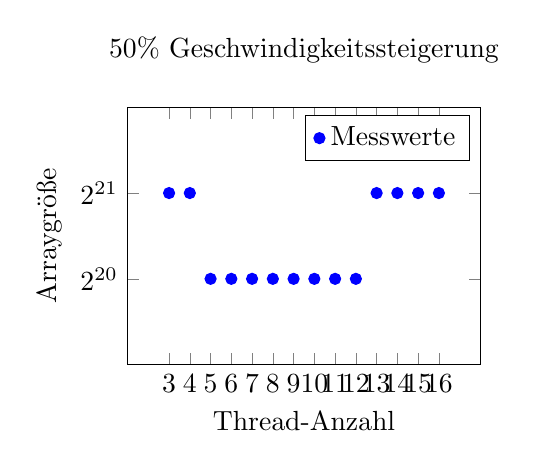
\begin{tikzpicture}
        \begin{axis}[
                title style={yshift=1.5ex},
                width=0.5\textwidth,
                height=0.4\textwidth,
                xlabel={Thread-Anzahl},
                ylabel={Arraygröße},
                title={50\% Geschwindigkeitssteigerung}, % Zeitpunkt der 50\% Geschwindigkeitssteigerung (incAray)
                xmin=1, xmax=18,
                ymin=2^19, ymax=2^22,
                grid style=dashed,
                legend pos=north east,
                ymode=log,
                log basis y=2,
                xtick={3,...,16},               % jeden Integer von 2 bis 17
                ytick={2^20,2^21},      % gewünschte y-Werte
                % yticklabels={\ensuremath{2^{19}},\ensuremath{2^{20}},\ensuremath{2^{21}},\ensuremath{2^{22}},\ensuremath{2^{23}}} % Beschriftung
            ]
            \addplot[only marks, blue, mark=*] coordinates {
                    (1,2)
                    (3,2097152)
                    (4,2097152)
                    (5,1048576)
                    (6,1048576)
                    (7,1048576)
                    (8,1048576)
                    (9,1048576)
                    (10,1048576)
                    (11,1048576)
                    (12,1048576)
                    (13,2097152)
                    (14,2097152)
                    (15,2097152)
                    (16,2097152)
                };
            \addlegendentry{Messwerte}
        \end{axis}
    \end{tikzpicture}%
}

\newcommand{\InkrementArrayDiagrammB}{%
    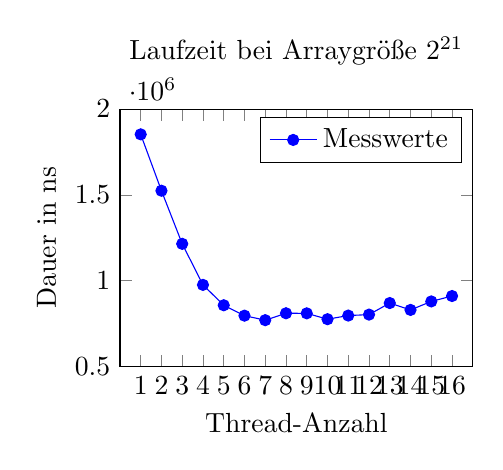
\begin{tikzpicture}
        \begin{axis}[
                title style={yshift=1.5ex},
                width=0.5\textwidth,
                height=0.4\textwidth,
                xlabel={Thread-Anzahl},
                ylabel={Dauer in ns},
                title={Laufzeit bei Arraygröße $2^{21}$},
                xmin=0, xmax=17,
                ymin=0.5*10^6, ymax=2*10^6,
                grid style=dashed,
                legend pos=north east,
                xtick={1,...,16},
                % ymode=log,
            ]
            \addplot[blue, mark=*] coordinates {
                    (1,1852600)
                    (2,1524000)
                    (3,1214400)
                    (4,975200)
                    (5,856500)
                    (6,795800)
                    (7,769500)
                    (8,809800)
                    (9,809400)
                    (10,775200)
                    (11,796400)
                    (12,802000)
                    (13,869400)
                    (14,829300)
                    (15,878800)
                    (16,910300)
                };
            \addlegendentry{Messwerte}
        \end{axis}
    \end{tikzpicture}%
}

\newcommand{\InkrementArrayDiagrammC}{%
    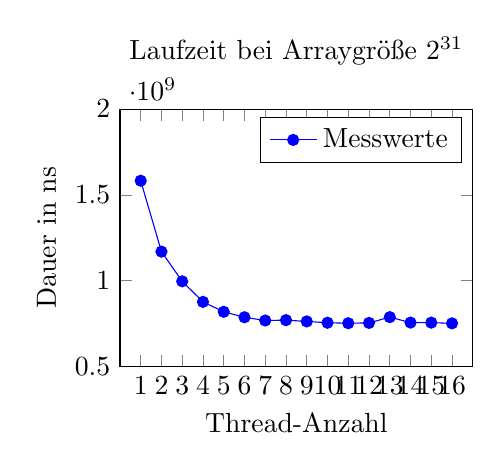
\begin{tikzpicture}
        \begin{axis}[
                title style={yshift=1.5ex},
                width=0.5\textwidth,
                height=0.4\textwidth,
                xlabel={Thread-Anzahl},
                ylabel={Dauer in ns},
                title={Laufzeit bei Arraygröße $2^{31}$}, % ($2^{31}-1$)
                xmin=0, xmax=17,
                ymin=0.5*10^9, ymax=0.2*10^10,
                grid style=dashed,
                legend pos=north east,
                xtick={1,...,16},
            ]
            \addplot[blue, mark=*] coordinates {
                    (1,1582322800)
                    (2,1169109200)
                    (3,995920200)
                    (4,876230000)
                    (5,818310300)
                    (6,786585300)
                    (7,767543800)
                    (8,769668500)
                    (9,762244800)
                    (10,754572500)
                    (11,751793100)
                    (12,753548100)
                    (13,787192000)
                    (14,755368000)
                    (15,755257400)
                    (16,751066600)
                };
            \addlegendentry{Messwerte}
        \end{axis}
    \end{tikzpicture}%
}

\newcommand{\InkrementArrayDiagrammD}{%
    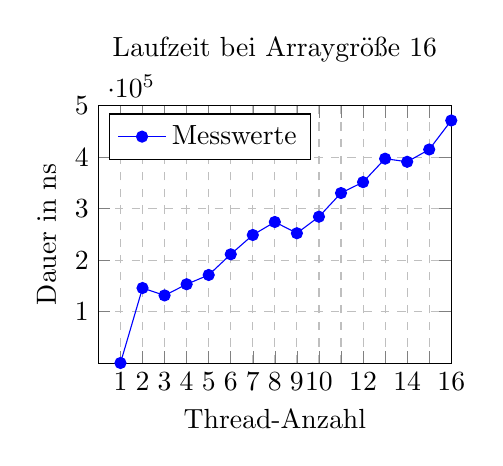
\begin{tikzpicture}
        \begin{axis}[
                title style={yshift=1.5ex},
                width=0.5\textwidth,
                height=0.4\textwidth,
                xlabel={Thread-Anzahl},
                ylabel={Dauer in ns},
                title={Laufzeit bei Arraygröße 16},
                grid=both,
                grid style=dashed,
                xmin=0, xmax=16,
                ymin=0, ymax=5*10^5,
                grid style=dashed,
                legend pos=north west,
                xtick={1,...,16},
                ytick={1*10^5,2*10^5,3*10^5,4*10^5,5*10^5},
                xticklabels={$1$,$2$,$3$,$4$,$5$,$6$,$7$,$8$,$9$,$10$,$ $,$12$,$ $,$14$,$ $,$16$},
            ]
            \addplot[blue, mark=*] coordinates {
                    (1,200)
                    (2,145900)
                    (3,131500)
                    (4,153200)
                    (5,171200)
                    (6,211400)
                    (7,248900)
                    (8,274200)
                    (9,252300)
                    (10,284400)
                    (11,330400)
                    (12,351600)
                    (13,397200)
                    (14,391100)
                    (15,415000)
                    (16,471400)
                };
            \addlegendentry{Messwerte}
        \end{axis}
    \end{tikzpicture}%
}

\newcommand{\InkrementArrayDiagrammE}{%
    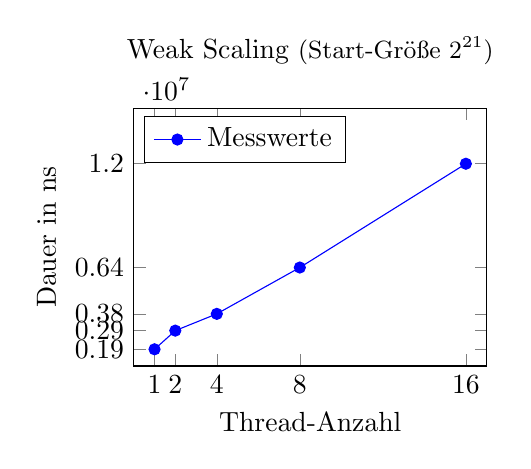
\begin{tikzpicture}
        \begin{axis}[
                title style={yshift=1.5ex},
                width=0.5\textwidth,
                height=0.4\textwidth,
                xlabel={Thread-Anzahl},
                ylabel={Dauer in ns},
                title={Weak Scaling {\small (Start-Größe $2^{21}$)}}, % Threads und Länge verdoppeln
                xmin=0, xmax=17,
                ymin=1*10^6, ymax=1.5*10^7,
                grid style=dashed,
                legend pos=north west,
                xtick={1,2,4,8,16},
                ytick=data,
            ]
            \addplot[blue, mark=*] coordinates {
                    (1,1910700)
                    (2,2925400)
                    (4,3837500)
                    (8,6358100)
                    (16,12003500)
                };
            \addlegendentry{Messwerte}
        \end{axis}
    \end{tikzpicture}%
}

\newcommand{\InkrementArrayDiagrammF}{%
    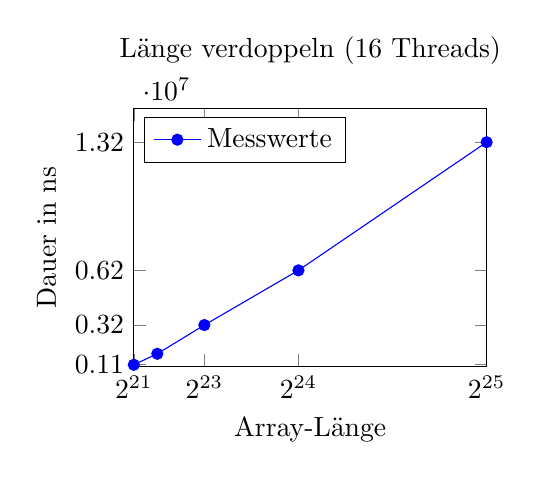
\begin{tikzpicture}
        \begin{axis}[
                title style={yshift=1.5ex},
                width=0.5\textwidth,
                height=0.4\textwidth,
                xlabel={Array-Länge},
                ylabel={Dauer in ns},
                title={Länge verdoppeln (16 Threads)},
                xmin=2^21, xmax=1 * 2^25,
                ymin=1*10^6, ymax=1.5*10^7,
                grid style=dashed,
                legend pos=north west,
                xtick={2^21,2^23,2^24,2^25},
                xticklabels={$2^{21}$, $2^{23}$, $2^{24}$, $2^{25}$},
                scaled x ticks=false,
                ytick={1077100,3237700,6213600,13184900},
            ]
            \addplot[blue, mark=*] coordinates {
                    (2097152,1077100)
                    (4194304,1675200)
                    (8388608,3237700)
                    (16777216,6213600)
                    (33554432,13184900)
                };
            \addlegendentry{Messwerte}
        \end{axis}
    \end{tikzpicture}%
}

\newcommand{\InkrementArrayText}{
    Anhand dieses einfachen Beispiels soll gezeigt werden, was Parallelisierung in der Praxis bewirkt und dass die Praxis nicht immer mit den Erwartungen übereinstimmt. Zudem stellt dieses Beispiel einen guten Einstieg in das Thema Parallelisierung dar.
    An den Diagrammen ist deutlich zu erkennen, dass dieses Beispiel nicht linear mit der Thread-Anzahl skaliert, obwohl dies rein theoretisch zu erwarten wäre. Dies liegt wahrscheinlich daran, dass das Datenübertragungslimit erreicht ist. Dies würde erklären, warum ab einem gewissen Punkt mehr ausgelastete Kerne keinen weiteren Performancegewinn mehr bringen. Zudem ist zu erkennen, dass das Array mindestens $2^{20}$ groß sein muss, damit eine parallele Ausführung einen mindestens zweifachen Geschwindigkeitsvorteil gegenüber der seriellen Laufzeit erreicht.
    Zusätzlich ist anzumerken, dass die serielle Laufzeit dieser Funktion normalerweise unter 100~ns liegt. Dies ist auf Compiler-Optimierungen zurückzuführen. Daher wurde diese Funktion mit \texttt{volatile} ausgeführt, was verhindert, dass der Compiler die eigentliche Aufgabe herausoptimiert und sie somit messbar bleibt. Das \texttt{volatile}-Schlüsselwort sorgt dafür, dass bei jedem Lesevorgang die Daten aus dem RAM geladen werden müssen. Daher ist es auch das wahrscheinlichste Szenario, dass dieses Beispiel durch das Datenratenlimit begrenzt ist. Zusätzlich ist die eigentliche Aufgabe trivial für die CPU und lastet diese daher nicht vollständig aus.
}



\newcommand{\InkrementArray}{
    % Inkrement-Array
    \InkrementArrayText
    \newline
    \InkrementArrayDiagrammA
    \InkrementArrayDiagrammD
    \newline
    \InkrementArrayDiagrammB
    \InkrementArrayDiagrammC
    \newline
    \InkrementArrayDiagrammE
    \InkrementArrayDiagrammF
}